\documentclass[11pt,letterpaper]{article}
\usepackage[T1]{fontenc}
\usepackage{lmodern,amsmath,amssymb,booktabs,array,geometry,xcolor,microtype,graphicx}
\usepackage{fancyhdr,pgfplots}
\pgfplotsset{compat=1.18}
\usepackage{hyperref}
\geometry{left=.95in,right=.95in,top=.83in,bottom=.85in,headheight=15pt,headsep=15pt}
\definecolor{ink}{HTML}{1D3C4C}
\definecolor{blue}{HTML}{236287}
\definecolor{warm}{HTML}{A45131}
\hypersetup{colorlinks=true,linkcolor=blue,urlcolor=blue,pdftitle={Unpredictability and the transfer of power}}
\pagestyle{fancy}\fancyhf{}
\fancyhead[L]{\small\sffamily\color{ink}Unpredictability and the transfer of power}
\fancyhead[R]{\small\sffamily\color{ink}Research note}
\fancyfoot[C]{\small\sffamily\thepage}
\renewcommand{\headrulewidth}{.25pt}
\setlength{\parindent}{0pt}\setlength{\parskip}{5.3pt}
\setlength{\abovedisplayskip}{7pt}\setlength{\belowdisplayskip}{7pt}
\setlength{\abovedisplayshortskip}{4pt}\setlength{\belowdisplayshortskip}{4pt}
\setlength{\emergencystretch}{2em}
\newcommand{\sect}[1]{\section*{\color{ink}#1}}
\newcommand{\lead}[1]{\textbf{#1}\enspace}
\newcommand{\E}{\mathbb E}
\newcommand{\Var}{\operatorname{Var}}
\newcommand{\Prb}{\operatorname{Pr}}
\newcommand{\src}[2]{\href{#1}{#2}}
\begin{document}
\thispagestyle{plain}
{\small\sffamily\color{ink}Research note for Kun Heo \hfill Revised 24 November 2026}\par
{\LARGE\bfseries\color{ink}Unpredictability and the transfer of power\par}
{\large Ideological competition and learning from implemented policies\par}
\vspace{3pt}

Two voters favor the same amount of bank support in ordinary times. One thinks that expanding the facility in a crisis prevents otherwise viable firms from failing. The other expects it mainly to protect insolvent banks. A promise to expand the facility following bad news can move their votes in opposite directions. If the facility is expanded, its actual performance also supplies evidence about the competing accounts. An election therefore allocates authority both to respond to future news and to choose which policies the electorate will get to learn about. Section 7 shows how this second consideration can change whether a defeated incumbent concedes.

\sect{1\quad A causal interpretation of responsiveness}
Let $x_0$ denote a publicly known reference policy, $\omega_t$ a mean-zero economic condition, and $Y_t$ a measured benefit relative to the reference. For the tractable version, use
\[
 Y_t=a_*(x_t-x_0)\omega_t+\varepsilon_t,\qquad
 u_i(x_t,Y_t)=-(x_t-\beta_i)^2+2\gamma_iY_t ,
 \qquad \varepsilon_t\sim N(0,\sigma_\varepsilon^2).
\]
The persistent parameter $a_*$ governs what additional intervention accomplishes under stress. The baseline $\beta_i$ and value $\gamma_i$ of the outcome are fixed. Measurement shocks are independent across observations and of the current state and policy choice. The material payoff is linear in the measured benefit and quadratic in the policy instrument. This choice preserves the draft's policy-distance calculation.

Before the election everyone knows the distribution of the government's eventual forecast $m_t=\E[\omega_t\mid\text{post-election report},H_t]$. Its variance conditional on the public history is $S_t$. The state and its report are independent of the causal map conditional on the public environment. Under the point model $a$, player $i$'s preferred policy for the current term is
\[
 x^{\mathrm{flow}}_i(m_t;a)=\beta_i+\gamma_i a\,m_t,\qquad
 \alpha_{i,t}=\gamma_i a .
\]
Thus people can agree on both $\beta_i$ and $\gamma_i$ and want different responses because they adopt different causal models. For a given affine governing rule $x_h=\beta_h+\alpha_hm_t$, expected loss relative to $i$'s preferred current rule is exactly
\[
 \Lambda_i^h=(\beta_i-\beta_h)^2+S_t(\alpha_{i,t}-\alpha_h)^2 .
\]
This follows by completing the square conditional on $m_t$ and integrating using $\E m_t=0$. Holding today's adopted model and the candidates' rules fixed recovers the draft's realignment mechanism. Changing the record or the models offered can also change $\alpha_{i,t}$. An officeholder choosing policy for its future informational consequences can depart from her flow optimum.

\newpage
\sect{2\quad What the parties offer and what voters adopt}
Each democratic term starts with a public policy record $H_t$, an incumbent, and a known distribution of the news the next government will receive. The incumbent runs again and the opposition chooses a nominee. Once both nominees are known, the parties simultaneously offer causal models $a_L,a_R$. The voter then obtains her own observation of the consequences of a previously implemented policy. With voter-specific experiences, citizens can see different fits even when they share a public history. A party's claim about how intervention works and its nominee's governing rule are separate objects.

Write $z_s=(x_s-x_0)\omega_s$. With independent Gaussian errors of equal variance, citizen $i$ selects the offered model that minimizes
\[
 \sum_{s\in H_{it}}(Y_s-a z_s)^2,\qquad a\in\{a_L,a_R\},
\]
where $H_{it}$ includes her private observation. Split exact ties by an independent fair draw. The test scores predictions conditional on the policies implemented. A voter can adopt the right's explanation and elect the left if its nominee is closer in baseline or in its actual response. Izzo, Martin, and Callander model strategic party supply, likelihood-based adoption and subsequent electoral choice. Their supplement already treats reassessment after further outcomes. \src{https://doi.org/10.1111/ajps.12763}{Izzo, Martin, and Callander (2023)} and \src{https://www.federicaizzo.com/pdf/Ideological_Competition_FINAL_Website.pdf}{online appendix E.4}.

\lead{A tractable ideological contest.} Consider a final, lawfully enforced election with one decisive voter of known baseline and $\gamma_i>0$, fixed and publicly understood affine candidate rules for the term, and $\alpha_r>\alpha_l$. Each party assigns a fixed positive value to its candidate's victory, independent of the voter's private outcome, as when it cares directly about the specified policy rule and office. There is an independent additive uniform valence shock with density $\phi$, and all feasible winning probabilities are interior. Conditional on adoption of $a$, the right's winning probability is affine in $a$ with coefficient
\[
 2\phi S_t\gamma_i(\alpha_r-\alpha_l).
\]
Let $X=\sum_{s\in H_{it}}z_sY_s/\sum_{s\in H_{it}}z_s^2$ have a common predictive normal distribution for the parties, with median $\mu$ and density $f$. A private normal outcome at a fixed nonzero $z$ gives this case when its predictive distribution is Gaussian. The voter picks the proposal closer to $X$. For $S_t>0$, the left minimizes and the right maximizes the expected adopted coefficient. If the feasible interval contains the interior solution, the equilibrium offers are
\[
 a_L^*=\mu-\frac{1}{2f(\mu)},\qquad a_R^*=\mu+\frac{1}{2f(\mu)}.
\]
To see this, set $c=(a_L+a_R)/2$. The expected adopted coefficient is $a_L F(c)+a_R[1-F(c)]$. The two first-order conditions give $F(c)=1/2$ and $(a_R-a_L)f(c)=1$. The increasing normal hazard and its reflected counterpart make each best response unique on its ordered side. Crossing the rival's proposal moves the adopted coefficient weakly to the wrong side of it.

The gap is the scalar ideological contest of Izzo, Martin, and Callander under this electoral payoff. Holding history fixed, an increase in $S_t$ raises the electoral reward to persuading the voter while leaving the equilibrium offers fixed. At $S_t=0$ the contest has no electoral stakes here. With endogenous governing rules or constitutional risk, the affine winning-probability argument can cease to apply.

\newpage
\sect{3\quad How governing produces the next record}
After the certified election and any transfer dispute, the actual officeholder sees the state report, chooses $x_t$, and generates $Y_t$. The implemented policy, eventual realized state, and measured outcome enter the next public record under either regime. Outcomes from policies passed over are unavailable. In the earlier specification $Y=x-b-a\omega+\varepsilon$, anyone observing $x$ could subtract it and learn equally much about $a$ regardless of who governed. Here the distribution of the evidence depends on the policy selected.

\lead{Disagreement about linear returns.} Take two proposed coefficients, $a$ and $b$. If $a$ is true, then conditional on the implemented $x$ and realized $\omega$ the expected log-likelihood advantage of $a$ over $b$ from this observation equals
\[
 \mathbb E_a\!\left[\log\frac{p_a(Y\mid x,\omega)}{p_b(Y\mid x,\omega)}
       \,\middle|\,x,\omega\right]
   =\frac{(a-b)^2(x-x_0)^2\omega^2}{2\sigma_\varepsilon^2}.
\]
It follows directly from the KL divergence of two normals with equal variance. An entire term at $x_0$ supplies no public evidence from the implemented policy about this disagreement, even if the economy experiences a large shock. A single informative experiment can favor the incorrect model by chance. For a Bayesian observer with variance $v$ and a normal prior immediately before the observation, posterior precision increases by $(x-x_0)^2\omega^2/\sigma_\varepsilon^2$. This Bayesian calculation describes learning by the policymaker. Citizens can still use the party-model selection rule on page 2.

For an illustration, let $\omega=\pm\sqrt{V}$ with equal probabilities, and let the pre-policy signal reveal it with probability $r$ and otherwise be uninformative. Then $S=rV$. Holding the identity of the ruler and its affine rule fixed,
\[
 \E\big[(x_h-x_0)^2\omega^2\big]
    =V\big[(\beta_h-x_0)^2+\alpha_h^2 S\big].
\]
At the same $S$, raising $V$ from 1 to 4 and lowering $r$ from $.8$ to $.2$ leaves the current candidate comparison unchanged and multiplies expected evidence by four whenever that evidence is positive. At fixed $V$, better reporting also speeds learning when $h$ actually responds to the report. At the same baseline $x_0$, two governments with different $|\alpha_h|$ generate different amounts of evidence even if they receive identical news. Expectations of these differences can affect a forward-looking vote or concession decision immediately.

\lead{The political feedback.} The next election starts from the policies the previous government had reason to try. A government that repeatedly chooses interventions on which competing accounts make similar predictions can leave their disagreement unresolved. A government that implements interventions with sharply different predicted consequences can create evidence that changes which account people adopt. The likelihood formula identifies the amount of discrimination between specified models. The direction in which voters update depends on the realized outcome, and parties may change their next proposals.

\newpage
\sect{4\quad Learning about policies and about ideologies}
Callander models an unknown persistent mapping from policies to outcomes. Implementing a policy reveals information about that point of the map and, through correlation, about nearby policies. The linear specification on page 1 uses the same feedback channel with a single unknown coefficient. To allow different policy intensities to have local effects, draw the entire map once as follows.
\[
 Y_t=\omega_t F_*(x_t)+\varepsilon_t,\qquad
 \mathcal M_a:\quad F(x)=a(x-x_0)+\nu W(x-x_0),\qquad \nu>0.
\]
Here $W$ is one persistent two-sided standard Brownian path anchored at $x_0$. The parties offer different drifts $a_L,a_R$ and agree on roughness $\nu$. Score the predictive likelihood of the entire record under each model, conditioning on earlier observations of the same map. \src{https://doi.org/10.1257/aer.101.6.2277}{Callander (2011), \emph{Searching and Learning by Trial and Error}}, and \src{https://doi.org/10.1017/S0003055411000426}{\emph{Searching for Good Policies}.}

\lead{Inside the tested range.} Suppose two adjacent tried policies $\ell<u$ have exactly known effects $F(\ell),F(u)$, as with noiseless historical measurements. For any $\ell<x<u$, both models predict a Brownian bridge with mean and variance
\[
 \frac{u-x}{u-\ell}F(\ell)+\frac{x-\ell}{u-\ell}F(u),\qquad
 \nu^2\frac{(x-\ell)(u-x)}{u-\ell}.
\]
The drift cancels. Observing the new policy can improve knowledge of its effect while contributing exactly zero log-likelihood evidence between these two ideologies. This remains true for an independently noisy new observation when the bracketing effects are known exactly.

\lead{Beyond the tested range.} Beyond the outermost tried policy $u$, at distance $d>0$, the two predicted means are $F(u)+a_Ld$ and $F(u)+a_Rd$. With the same noise variance as before, the expected log-likelihood advantage under either true model over its rival is
\[
 \frac{\omega^2(a_R-a_L)^2 d^2}{2(\sigma_\varepsilon^2+\omega^2\nu^2d)}.
\]
For an exactly observed map value and nonzero $\omega$, this is $(a_R-a_L)^2d/(2\nu^2)$. The exact inside/outside distinction uses known bracketing points and common roughness. Noisy historical endpoints or competing models of local curvature can make interior observations politically informative too.

\begin{center}
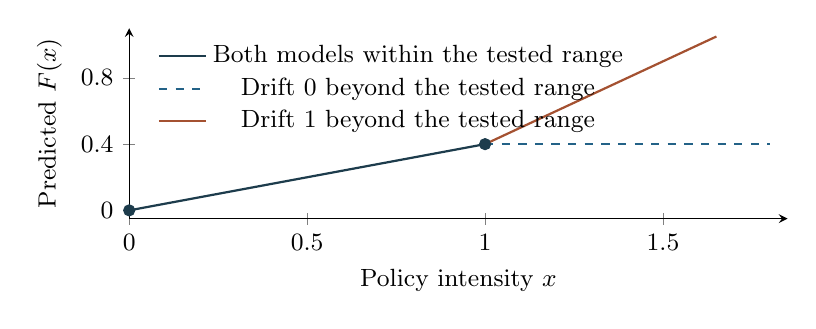
\begin{tikzpicture}
\begin{axis}[width=.82\linewidth,height=4cm,axis lines=left,xmin=0,xmax=1.85,ymin=-.05,ymax=1.1,
 xlabel={Policy intensity $x$},ylabel={Predicted $F(x)$},xtick={0,.5,1,1.5},ytick={0,.4,.8},
 tick label style={font=\small},label style={font=\small},legend style={font=\small,draw=none,at={(.03,.97)},anchor=north west,fill=none}]
\addplot[thick,color=ink,domain=0:1] {.4*x};\addlegendentry{Both models within the tested range}
\addplot[thick,color=blue,dashed,domain=1:1.8] {.4};\addlegendentry{Drift 0 beyond the tested range}
\addplot[thick,color=warm,domain=1:1.65] {.4+(x-1)};\addlegendentry{Drift 1 beyond the tested range}
\addplot[only marks,mark=*,color=ink] coordinates {(0,0) (1,.4)};
\end{axis}
\end{tikzpicture}
\end{center}

\newpage
\sect{5\quad How the tested range disciplines ideological offers}
The path model connects the content of the public record directly to the competition between parties. Order exactly known policy effects from the lowest to the highest tried intensity, including the known reference $x_0$. Write $D=x_{\max}-x_{\min}$ for the width of the range and $\Delta F=F(x_{\max})-F(x_{\min})$. Brownian increments on disjoint intervals are independent. The log likelihood of drift $a$ is, up to terms independent of $a$,
\[
 -\sum_k\frac{(\Delta F_k-a\Delta x_k)^2}{2\nu^2\Delta x_k}
 =\frac{a\Delta F}{\nu^2}-\frac{a^2D}{2\nu^2}+\mathrm{constant}.
\]
The record can include many policies. Its information about a constant drift is $D/\nu^2$. Additional trials between known endpoints can help future governments select good local policies, even though the public likelihood comparison between drifts stays exactly the same.

\lead{A joint electoral result.} Set $x_0=0$ and suppose the public record covers $[-D,0]$. Before the election, each party proposes a drift. The decisive voter privately observes a result from a previously implemented trial to the left of $-D$. With independent Gaussian measurement error $\eta$, its increment in increasing policy order has distribution
\[
 Z=F(-D)-F(-D-d)+\eta,\qquad
 Z\mid a\sim N(ad,V_d),\qquad V_d=\nu^2d+\Var(\eta),\quad d>0.
\]
Let both current candidates' future policy rules lie on the untested positive side, and let the right be more responsive. Conditional on a drift, Brownian increments on that side are independent of the earlier left-side observations. Each model therefore predicts mean $a x$ for the policies being voted on. The rule comparison and the uniform-valence electoral coefficient on page 2 follow exactly. This one-sided history gives a tractable case in which both mechanisms operate in the same contest.

Combining the public and private likelihoods, the voter adopts the offer closest to
\[
 X=\frac{\Delta F/\nu^2+dZ/V_d}{D/\nu^2+d^2/V_d}.
\]
For example, let parties have normal prior variance $v_0$ on the true drift, updated only with the public record before offers. Their posterior variance is $v_D=(v_0^{-1}+D/\nu^2)^{-1}$. Their predictive variance for $Z$ is $V_d+d^2v_D$. With constant stakes in victory as on page 2, the equilibrium gap between offers is
\[
 a_R^*-a_L^*
 =\sqrt{2\pi}\,
   \frac{d\sqrt{V_d+d^2v_D}/V_d}{D/\nu^2+d^2/V_d}.
\]
This is the earlier $1/f(\mu)$ formula evaluated at the density of the history-dependent $X$. Holding the private trial's design fixed, a wider public range strictly reduces the gap. Its denominator increases and the predictive variance in its numerator falls. Conditional on that same public range and record, increasing $S_t$ increases the electoral value of winning the ideological contest. Thus a narrowly tested policy domain can leave wide divergence over causal models precisely when an anticipated crisis makes the choice between them electorally consequential. This is a final-election result with fixed rules, common roughness and interior valence probabilities.

\newpage
\sect{6\quad What changes in the transfer game}
Terms repeat with common discount factor $\delta\in(0,1)$. The two parties value policy and office. The sitting president personally decides whether to concede. Potential officeholders and parties evaluate consequences with a specified common Bayesian prior over the map. They condition on relevant public evidence, including electoral outcomes if informative. The parties have no additional private information about the map when offering interpretations. Voters and organized blocs use the adopted model to forecast material payoffs along the anticipated strategies. At future decisions they can adopt another model as the record changes. For a current choice, compare both branches under the same current model, allowing for these future choices.

\lead{Timing within a democratic term.}
\begin{enumerate}
\setlength{\itemsep}{1pt}
\item Observe the incumbent, the policy record, and the upcoming signal technology. The opposition chooses a challenger and both parties offer interpretations of the record.
\item Citizens receive any new private experiences, choose a model by fit, observe the electoral shock, and vote. The result is publicly certified.
\item A losing incumbent concedes or attempts to remain. The organized blocs observe a refusal and the enforcement quorum and choose whether to act. A lawful transfer installs the winner. Successful subversion entrenches the incumbent and imposes the institutional loss $\chi_i$ per term.
\item The actual ruler sees the current state report and chooses policy. The realized state, the policy, and its measured outcome enter the next record. Elections continue under democracy. Policy feedback also continues under autocracy.
\end{enumerate}

Write $H$ for the full relevant history, including the public state and any actor-specific information when evaluating that actor's payoff. In the linear case the ruler's choice, up to current terms independent of $x$, solves
\[
 \max_x\,\left\{-(x-\beta_h)^2+2\gamma_h\bar a_h\,m_t(x-x_0)
       +\delta\,\E_h[V_h(H')\mid H,m_t,x,\text{regime}]\right\}.
\]
Here $\bar a_h$ is the ruler's posterior mean. In the path model replace $\bar a_h(x-x_0)$ by the conditional mean of $F(x)$. The continuation value depends on which experiment $x$ supplies. Even a correctly elicited preferred current response can therefore differ from the ruler's dynamic choice.

At a certified defeat, let $C_i^j(H)$ be the value of installing challenger $j$ lawfully and $A_i^I(H)$ the value of entrenching the incumbent $I$, including their respective policy choices and resulting public records. A bloc with cost $c_b$ is willing to enforce when pivotal exactly if $C_b^j-A_b^I\ge c_b$. With $q_I$ the resulting chance of successful entrenchment conditional on an attempt, refusal is optimal for the incumbent when
\[
 q_I(A_I^I-C_I^j)>(1-q_I)\kappa+k .
\]
Use the public coordination convention that implements an attainable enforcement quorum. The new term in the comparison is the difference in the value of the records that the two rulers will generate. A citizen may dislike the rival's policy but value the evidence it would produce. The sign depends in part on what a subsequent ruler would do with that evidence. Callander and Hummel show how a prospective successor can change today's incentive to experiment. \src{https://doi.org/10.3982/ECTA10616}{Callander and Hummel (2014).}

\newpage
\sect{7\quad A solved transfer with no immediate policy disagreement}
Suppose an incumbent $I$ has just lost to $j$. There are two policy terms left and one opportunity for subversion, now. The two officeholders have baseline $x_0=\beta_I=\beta_j=0$, no office rent, and different values of the outcome, $\gamma_I=1$ and $\gamma_j=0$. Both enter the decision with posterior $a_*\sim N(0,1)$ and unit measurement noise. Their immediate preferred policy is zero. The first state is $\omega_1=\pm1$ with equal probabilities and is revealed after the transfer decision. The first-term policy is the size $x\ge0$ of a pilot. In term two the ruler can choose any signed policy. Under orderly transfer a future election can return $I$ with a fixed probability independent of the record. The implemented pilot supplies the only subsequent evidence about $a_*$. Set $\delta=.8$ and $\Var(\omega_2)=5$. Vary the probability of an accurate second-term report between $.2$ and $1$, so $S_2=1$ or $5$.

Under a lawful transfer $j$ selects $x=0$. She values only the squared cost of policy, and zero policy in both terms is obtainable even if $I$ returns, because an uninformative pilot leaves its posterior mean at zero. Under entrenchment $I$ chooses the experiment and uses its results in the final term. Conditional on $x$ and $\omega_1$, its posterior mean is $\bar a_2=x\omega_1Y_1/(1+x^2)$ and its last policy is $\bar a_2m_2$. The expected two-term policy gain relative to the lawful branch is
\[
 \max_{x\ge0}\left[-x^2+\delta S_2\,\frac{x^2}{1+x^2}\right]
   =\big(\max\{0,\sqrt{\delta S_2}-1\}\big)^2.
\]
Indeed, the variance of the posterior mean across possible pilot outcomes is $x^2/(1+x^2)$. The optimal $x^2$ is $\max\{0,\sqrt{\delta S_2}-1\}$. More precise future monitoring increases the value of knowing how to respond to tomorrow's report and can make a costly pilot worthwhile today.

For the enforcement game take two blocs with identical $(\beta,\gamma)=(0,1)$, which have arrived at this history having adopted different models, $a=0$ and $a=1$. Each actor loses $.1$ per term under autocracy. Each bloc pays $.05$ to act. One bloc suffices with probability $1/2$ and both are needed otherwise. Attempt and failure costs are each $.1$.
\begin{center}\small
\begin{tabular}{@{}lrr@{}}\toprule
After the same certified defeat & $S_2=1$ & $S_2=5$\\\midrule
Pilot under lawful transfer / under entrenchment & $0\,/\,0$ & $0\,/\,1$\\
Incumbent's $A_I^I-C_I^j$ & $-.18$ & $.82$\\
Bloc's $A_b^I-C_b^j$ under $a=0$ / under $a=1$ & $-.18\,/\,-.18$ & $-2.18\,/\,.82$\\
Takeover probability given an attempt & $0$ & $.50$\\
Net gain from refusing & $-.20$ & $.26$\\\bottomrule
\end{tabular}
\end{center}
For example, when $x=1$, a bloc holding model $a$ forecasts a final posterior mean with mean $a/2$ and variance $1/4$. Its expected policy gain is $-1+\delta S_2(3a^2-1)/4$. Subtract $(1+\delta).1$ for the regime loss. Only the $a=0$ bloc will defend at high $S_2$. These are equilibrium choices in the post-defeat subgame, conditional on the given adoption history. The equilibrium determination of the initial election and these particular offers remains open in this example. The strategic contest on page 2 and the independent-feedback equilibrium in Appendix D have their own stated assumptions.

\newpage
\sect{8\quad Testing the amendment}
The observable distinction is between the response a voter wants, what she thinks a policy will accomplish, and the actions that could change her mind. In an employment or banking vignette, elicit four state-contingent ideal policies in common units, then ask for outcome forecasts under \emph{each} policy at the \emph{same} state. Two respondents can favor exactly the same policy today and predict different consequences from intervening during a downturn. Separately eliciting which outcome each respondent values helps distinguish $\gamma_i$ from her adopted model. Elicit party identity before treatments.

\lead{Future state news and the current vote.} Cross state variance $V\in\{1,4\}$ with a common post-election reveal probability $r\in\{.2,.8\}$. The forecast variance is $S=rV$. With predetermined rules, a one-term choice and a common ideological record, the two arms $(1,.8)$ and $(4,.2)$ imply equal utility comparisons. The response to the high-$S$ arm has opposite signs for voters closer in responsiveness to different candidates. Estimate within-country effects in the United States and South Korea. Probability magnitudes require a specified choice-noise model.

\lead{Whose explanation gains support?} Elicit forecasts before presenting a realized policy outcome. Randomize assignment to a record from the reference policy or from a policy on which the two models give substantially different forecasts. Give respondents enough information to interpret which policy was implemented and the conditions in force. Their relative likelihoods predict which account gains support after a particular outcome. Independently record which party the respondent then chooses. These are distinct outcomes. In the Brownian specification, a second task can provide exact outcomes at two bracketing policies and compare a new trial inside and beyond the tested range. Elicit both the estimated local effect and the credibility of rival general claims. The model predicts that an interior result can change the former while leaving the latter unchanged.

\lead{Concession and the evidence a successor would produce.} Independently assign a certified defeat. Keep the lawful winner's label, baseline policy, and present conditions fixed. Vary which pilot it would conduct, whether the outcome will be observed before a later policy choice, and, in a separate treatment, the incumbent's chance of a lawful return. A pilot costs something and its policy consequences can matter directly. Include an otherwise identical arm in which the result arrives only after the last policy decision. The interaction with timely feedback isolates the instrumental value of the evidence under the maintained exclusion that publication timing has no effect on direct payoffs or institutional costs. Separate perceived validity of the count, recognition of the winner, and willingness to incur a specified cost to defend transfer.

The inequalities in these designs have different scopes. Equal present-election comparisons require equal continuations or a one-term task. The fourfold difference in expected evidence on page 3 requires the same known affine rule in both arms. The exact inside/outside comparison on page 4 requires known bracketing outcomes. The transfer calculation on page 7 conditions on an electoral and ideological history. None of the polling tabulations in Appendix E identifies these causal effects.

The following appendices retain the verified independent-feedback benchmark and the empirical context for the project. They document what follows with predetermined information transitions. In the amended game implemented policy changes those transitions, and equilibrium nominations, efforts to stay in office, and the long-run distribution of beliefs must be evaluated jointly.

\newpage
\sect{A\quad Hardening in the original nomination equilibrium}
Write $S=\Var(\E[\omega\mid m])$, where $m$ is news that the next government receives before acting. Write $d_b=\beta_R-\beta_L$ and $d_a=\alpha_R-\alpha_L$ for differences between the parties. In the draft's symmetric nomination equilibrium the candidates' midpoint is the median type $M$. With $g_i=U_i^r-U_i^l$ oriented toward $R$,
\begin{equation}
 g_i(S)=2w(S)\{d_b(\beta_i-\beta_M)+S d_a(\alpha_i-\alpha_M)\}.
\end{equation}
Set $\Lambda=d_b^2+Sd_a^2$. Differentiating $(1+2\phi B)w+2\phi\Lambda w^2=1$ gives
\[
 (Sw)'=w\frac{1+2\phi d_b^2 w^2}{1+2\phi\Lambda w^2}>0,
 \qquad
 \frac{g_i(S)}{\sqrt S}\longrightarrow
 \sqrt{2/\phi}\,\operatorname{sgn}(d_a)(\alpha_i-\alpha_M),\quad d_a\ne0.
\]
Thus some cross-pressured voters first approach indifference and switch. Eventually attachment grows for every fixed voter off the median responsiveness. A bounded valence shift $v$ moves mass $O(|v|/\sqrt S)$, since the indifference strip has width $|v|/[2w\sqrt{d_b^2+S^2d_a^2}]$ and the type density and support are bounded. The sign change of an individual comparison survives nomination because $w>0$. In this symmetric benchmark each side still wins half of elections. An electoral advantage for one side requires an asymmetry. Bimodality or the electoral collapse of a centrist party requires additional structure.

Two qualifications matter for interpretation. The movable share need not fall at every $S$, and the interior winning-probability effect of a common valence shift is still $\phi v$ in magnitude. Also, $S\leq\Var(\omega)$, so divergence is a statement across environments with sufficiently large underlying variance. A change in information alone can cross a political threshold at finite $S$.

\lead{Party and officeholder incentives.} The party values governing through its nominee by $B+w\Lambda$. The nominee's personal one-term policy gain from governing instead of her rival is $D^*=w^2\Lambda\to1/(2\phi)$. The party can have unbounded policy stakes while its candidate has bounded stakes. A sitting president's refusal therefore needs its own incentive constraint.

\newpage
\sect{B\quad Enforcement with policy-independent feedback}
Dates are infinite. The public state is the regime, the incumbent officeholder $I$, and an information environment $s$ with Markov kernel $P$. The two parties, their potential nominees, voters, and organized electoral constituencies are distinct long-lived players. At each democratic date the incumbent runs again. The opposition party chooses a challenger $j$ from its pool. Voters observe the candidates, the environment, and the electoral shock. The certified result is public. A winning incumbent governs. A losing incumbent can concede or attempt to retain office. Attempts cost $k$, and failed attempts also cost the incumbent $\kappa$. A successful takeover makes $I$ the permanent officeholder. The same state process and opportunities to learn about policy operate in both regimes.

If $h$ governs, let $u_i^h(s)$ include policy utility and any office rent. One may subtract $i$'s payoff under her own ideal rule from every flow, since its entire expected discounted stream is independent of political choices here. Autocracy additionally costs player $i$ an amount $\chi_i$ per period. Let $V_i(h,s)$ be the value at the beginning of a democratic date with incumbent $h$. For any function $f$, $Pf(s)=\E[f(s')\mid s]$. The values of a lawful term for $h$ and of immediate entrenchment by $h$ are
\begin{align}
 C_i^h(s)&=u_i^h(s)+\delta P V_i(h,\cdot)(s),\notag\\
 A_i^h(s)&=u_i^h(s)-\chi_i+\delta P A_i^h(s).
\end{align}
In the second line $P$ acts on the function $s\mapsto A_i^h(s)$. These are continuation values at the moment the result is known. The election winner governing today also becomes next period's incumbent.

\lead{Public enforcement.} An overt refusal is the common signal on which organized constituencies can coordinate, in the sense of Fearon (2011). After an attempt, a public draw specifies how many of $n$ finite blocs must endorse enforcement. If at least $m$ endorse, the lawful winner takes office. Each endorsing bloc pays $c_b>0$. A bloc would be willing to act if pivotal exactly when $C_b^j-A_b^I\ge c_b$. Let $N$ be the number of such blocs. An equilibrium that enforces the result exists exactly when $N\ge m$. With positive costs, exactly $m$ blocs act in any successful pure equilibrium. Each is pivotal. A public priority order selects those $m$. If $N<m$, all stay out. When $m>1$, collective inaction can also be an equilibrium even when enforcement is feasible. The construction uses the equilibrium that enforces whenever feasible. It models costly defense and acquiescence. Active pro-incumbent mobilization would require a separate action and incentive.

Let $q_I(s,j)=\Prb(m>N)$ be the takeover probability conditional on an attempt under this convention. Assuming the incumbent bears no bloc participation cost, the exact net gain from refusing is
\begin{equation}
 T_I(s,j)=q_I(s,j)\big[A_I^I(s)-C_I^j(s)\big]-(1-q_I(s,j))\kappa-k.
\end{equation}
A defeated incumbent refuses when $T_I>0$. This defines an observable meaning of radicalization for each side. It allows an incumbent to want to stay, its own voters to tolerate the violation, and the opposition still to enforce the result. A takeover requires an occasion to lose, an attempt, and successful entrenchment.

\newpage
\sect{C\quad The value of winning again}
There is a closed form for testing a peaceful democratic equilibrium. Hold the rules of the two officeholders fixed, and suppose all future transfers are honored. Let $p_I(s)$ denote the probability that $I$'s side wins a future lawful election in state $s$, independent of who currently holds office. Write $g_i^I(s)=u_i^I(s)-u_i^j(s)$ with $j$ the other side. Today, $I$ has already lost. Successful entrenchment replaces the lawful winner for sure this term, then only in future periods the incumbent's side would otherwise have lost. Thus
\begin{align*}
 A_i^I(s)-C_i^j(s)
  &=g_i^I(s)-\chi_i\\[-2pt]
  &\quad+\delta\big[P(\mathrm{Id}-\delta P)^{-1}
    \{(1-p_I)g_i^I-\chi_i\}\big](s).
\end{align*}
Here $\mathrm{Id}$ is the identity matrix and multiplication inside braces is state by state. In a stationary environment this reduces to
\begin{equation}
 A_i^I-C_i^j=\frac{(1-\delta p_I)g_i^I-\chi_i}{1-\delta}.
\end{equation}
For a voter who favors the incumbent, $g_i^I>0$. A higher probability of returning legally reduces the value of overturning today's loss by $\delta g_i^I/(1-\delta)$ per unit increase in $p_I$. A monitoring improvement on an issue on which the incumbent leads can increase both $g_i^I$ and $p_I$. The former raises the cost of leaving and the latter shortens the expected spell out of power. This makes the Przeworski--Rivero--Xi (2015) prospect of future victory an empirically distinct channel.

A bloc on the other side can become \emph{more} willing to defend the same transfer. A smaller cross-party defense coalition matters when the institutional quorum requires members of the incumbent's coalition. If the opposition can uphold the result alone, even unanimous acquiescence among incumbent supporters can coexist with a peaceful transfer. Low $S$ alone also guarantees little when baseline disagreement is already large.

\lead{Equilibrium with attempts.} Equation (4) evaluates a deviation from universal compliance. For positive on-path attempt rates, solve (2) using the actual regime transitions. Let $a\in\{0,1\}$ be the incumbent's best response after defeat, $d_i$ the expected bloc cost conditional on an attempt, and $t_i=k+(1-q_I)\kappa$ for the incumbent and zero for everyone else. With $p$ the incumbent's probability of a certified win, the value at a given nomination is
\[
 p C_i^I+(1-p)\big[C_i^j+a\{q_I(A_i^I-C_i^j)-d_i-t_i\}\big].
\]
Voters compare the two branches inside this expression, anticipating refusal. The opposition party chooses its nominee using its own value for the entire expression. Margins from a static election cannot simply be substituted when refusal occurs on path.

\lead{An incumbent who can change uncertainty.} The option to refuse adds $(1-p_I)\max\{0,T_I\}$ to the incumbent's ex ante value relative to conceding at that node. Where $T_I>0$, its derivative is $(1-p_I)T_I'-p_I'T_I$. Even if conditional refusal becomes more attractive, a higher reelection probability reduces the frequency with which the option is reached. If resistance strengthens, $q_I$ can fall as well. The draft's electoral result does not by itself sign this derivative.

\newpage
\sect{D\quad The independent-study benchmark}
This earlier infinite-horizon example uses an independent public study to resolve beliefs. The state of the world has mean zero and variance $5$ throughout. The post-election report reveals it with probability $.04$ or $.80$ and otherwise supplies no information, giving $S=.2$ or $4$. Conditional on beliefs about policy consequences remaining unresolved, the monitoring environment changes with transition rows $(.9,.1)$ and $(.3,.7)$, ordered low then high. Independently, at the end of each unresolved period a public study reveals the common causal slope with probability $.05$. This is the only feedback about that slope in this example. Before the study, the slope coordinates below are prior means. Afterward everybody agrees on the slope, so baseline differences alone determine policy comparisons at either level of monitoring. The study occurs under both regimes.

Each party has two potential officeholders. In coordinates $(\beta,\alpha)$ their types are $L_0=(0,0)$, $L_1=(.1,.1)$, $R_0=(1,1)$, and $R_1=(.9,.9)$. Party ideals are $(0,0)$ and $(1,1)$. The president personally chooses whether to concede. The opposition party chooses its nominee. The party in office and the individual officeholder each get a rent of $.2$. The discount factor is $.65$. Autocracy costs parties and potential officeholders $.45$ per period, and voters and blocs $2.1$. Attempt and failure costs are $.18$ and $.35$.

A publicly drawn decisive constituency replaces the draft's uniform electoral shock. The types $(0,0),(1,1),(.2,.8),(.8,.2)$ are decisive with probabilities $.25,.25,.35,.15$. Each maximizes its full continuation payoff. The blocs have types $(0,0)$ and $(1,1)$ and an endorsement cost of $.14$. One bloc can enforce the result with probability $.8$, and both are needed with probability $.2$. If either can act alone, the lawful winner's bloc has priority when willing.

\begin{center}
\small
\begin{tabular}{@{}lcccr@{}}
\toprule
&\multicolumn{3}{c}{Opposition's equilibrium nominee}&\\
\cmidrule(lr){2-4}
Incumbent & Low $S$, unresolved & High $S$, unresolved & Slope known & $T_I$, high unresolved\\
\midrule
$L_0$ & $R_1$ & $R_1$ & $R_0$ & $.736$\\
$L_1$ & $R_1$ & $R_1$ & $R_0$ & $.467$\\
$R_0$ & $L_0$ & $L_0$ & $L_0$ & $.973$\\
$R_1$ & $L_0$ & $L_1$ & $L_0$ & $.414$\\
\bottomrule
\end{tabular}
\end{center}

\lead{An equilibrium.} While the slope is disputed, the two cross-pressured constituencies switch in opposite directions as $S$ rises. The larger one moves from $L$ to $R$ even though $R$ is farther from its baseline. The chance of certifying $R$ rises from $.40$ to $.60$. Both switching groups still prefer a lawful transfer when their new favorite loses. At low $S$ both blocs would defend a transfer and either incumbent concedes ($T_I=-.530$). At high $S$ only the winning side's bloc would act. Either losing incumbent refuses, and four of five attempts fail.

After the public study, the chance of certifying $R$ returns to $.40$. Every incumbent concedes in a surviving democracy, even if monitoring stays high. A prior takeover remains irreversible. Starting unresolved with high monitoring, the probability of a takeover before the study is $.437$ under a left incumbent and $.410$ under a right incumbent. The corresponding one-period risks are $.12$ and $.08$.

The script \texttt{verify\_equilibrium.py} solves the twelve-state Bellman system in rational arithmetic. It checks each nomination deviation, voters' choices for each feasible nominee, and bloc and incumbent incentives. The strict inequalities persist in a neighborhood of the illustrated parameters under the specified enforcement convention. These are illustrative parameters.

\newpage
\sect{E\quad What the Korean data establish}
Gallup Korea asked whether respondents supported President Yoon Suk Yeol's impeachment following the December 2024 declaration of martial law. The table uses its published weighted percentages and contemporaneous party identification. The last column subtracts support among People Power Party (PPP) identifiers from support among Democratic Party (DP) identifiers.
\begin{center}\small
\begin{tabular}{@{}lrrrrrr@{}}\toprule
Field dates & Sample & All & PPP & DP & No party & DP less PPP\\\midrule
10--12 Dec 2024 & 1,002 & 75\% & 27\% & 97\% & 79\% & 70 pp\\
7--9 Jan 2025   & 1,004 & 64\% & 15\% & 99\% & 72\% & 84 pp\\
11--13 Feb 2025 & 1,004 & 57\% & 10\% & 98\% & 63\% & 88 pp\\\bottomrule
\end{tabular}\end{center}
The partisan gap widened by 18 percentage points between the selected December and February waves. The size of the PPP subgroup also changed, from 231 respondents in December to 396 in February. Repeated cross-sections combine individual opinion change with changes in who identifies with a party. Impeachment support measures willingness to remove the president, and the item elicits neither forecast variance nor mobilization. The open question is why supporters of the same party divided over removal, and whether expected policy under a successor explains that division. \src{https://www.gallup.co.kr/dir/GallupKoreaDaily/GallupKoreaDailyOpinion_606(20241213).pdf}{Gallup Korea 606}, \src{https://www.gallup.co.kr/dir/GallupKoreaDaily/GallupKoreaDailyOpinion_608(20250110).pdf}{608}, and \src{https://www.gallup.co.kr/dir/GallupKoreaDaily/GallupKoreaDailyOpinion_611(20250214).pdf}{611}. A survey directly addressing support for martial law offers a separate outcome. \src{https://doi.org/10.1177/00323217261462390}{Park and Chung (2026).}

\lead{Historical comparison.} The case coding changes what the model can explain.
\begin{center}\small\renewcommand{\arraystretch}{1.18}
\begin{tabular}{@{}>{\raggedright\arraybackslash}p{1.13in}p{4.94in}@{}}\toprule
Episode & Constitutional event and theoretical use\\\midrule
United States, 2020--21 & A sitting president lost reelection. Efforts to overturn the result preceded the transfer. This is the closest match to the post-defeat decision. \src{https://www.archives.gov/electoral-college/2020}{National Archives} and \src{https://www.govinfo.gov/app/details/GPO-J6-REPORT}{House Select Committee}.\\
South Korea, 2024--25 & A sitting president declared martial law during his term. The Assembly demanded its lifting, and an impeachment trial later removed him. This tests responses to an attack on a legislative check. \src{https://www.loc.gov/item/global-legal-monitor/2025-05-13/south-korea-constitutional-court-upholds-presidential-impeachment/}{Library of Congress}.\\
France, 1848--51 & Bonaparte's presidential victory in December 1848 came before the May 1849 legislative election. His 1851 coup arose under a constitutional bar to reelection. It speaks to a blocked route to retaining office. \src{https://www.assemblee-nationale.fr/dyn/histoire-et-patrimoine/deuxieme-republique/election-presidentielle-et-victoire-de-louis-napoleon-bonaparte}{Assembl\'ee nationale, 1848--49} and \src{https://www.assemblee-nationale.fr/dyn/histoire-et-patrimoine/deuxieme-republique/coup-d-etat-de-louis-napoleon-bonaparte}{1851}.\\
Weimar Germany & Nazi electoral gains preceded Hindenburg's appointment of Hitler as chancellor in January 1933. This is evidence about coalition change and accession through appointment. \src{https://encyclopedia.ushmm.org/content/en/article/hitler-comes-to-power}{US Holocaust Memorial Museum}.\\\bottomrule
\end{tabular}\end{center}
A broader model can let the public trigger be either a certified electoral defeat or a binding institutional check. For the latter, replace $C_i^j$ by the value of the legally available action with the incumbent still in office if the rule allows it. The policy stakes can concern a particular decision or the end of a term. The two triggers generate different observational risk sets.

\newpage
\sect{F\quad Observational evidence and paper architecture}
\lead{A regional or individual panel.} A panel can establish who switches and when. The British Election Study has a combined 2014--25 individual panel. In any US application, match respondents through an explicitly linked panel release and verify that the constitutional outcome was asked of the same people. Pre-shock geography and occupation can define exposed workers, indirectly exposed residents, and an unexposed comparison. Local demand, expectations of future income, migration, party cues, and the policy preferences of public workers or retirees can all change with exposure. The three groups alone do not isolate forecast spread. A recontact or new panel can measure baseline, responsiveness, expected successor policy, and perceived lawful return. To study nominations, code candidates' pre-election answers about what they would do under specific contingencies. An LLM can retrieve and provisionally code passages for bilingual human validation. Retain the original quotations and leave missing responses unscored. \src{https://pure.royalholloway.ac.uk/en/datasets/british-election-study-2014-25-combined-wave-1-30-internet-panel/}{British Election Study panel documentation.}

\lead{A more direct observational measure of $S$.} Fix an issue, a target date, and two policy-relevant information dates. Let $m_0$ be the forecast available at the first date and $m_1$ the forecast of the same target available at the second. For calibrated posterior means with nested information,
\[
 S_{0\to1}=\E[(m_1-m_0)^2\mid\mathcal F_0]
 =\Var(\omega\mid\mathcal F_0)-\E[\Var(\omega\mid\mathcal F_1)\mid\mathcal F_0].
\]
Estimate this conditional second moment from historical forecast vintages with comparable horizons, using only information available at the initial date. The signed revision is news. One realized squared revision is a noisy draw from the quantity of interest. A cross-section of forecasters disagreeing at one date is a different object. The Philadelphia Fed releases individual forecasts and probability distributions for selected US macroeconomic outcomes. Whether those forecasts approximate the government's information and voters' expectations of it is a substantive measurement question. \src{https://www.philadelphiafed.org/surveys-and-data/real-time-data-research/individual-forecasts}{Philadelphia Fed, individual forecasts} and \src{https://www.philadelphiafed.org/surveys-and-data/real-time-data-research/probability-variables}{probability variables}.

\lead{A country panel.} Country-report language in the World Uncertainty Index and administrative institutions in Brambor et al.'s state-capacity index have distinct units from forecast variance and the revealed share. Their interaction can be an exploratory correlate. Estimating separate hazards for an attempt and its success, with an explicit set of opportunities, is necessary to interpret an observed breakdown rate. Electoral defeats, midterm legislative checks, and term-limit confrontations require separate denominators. \src{https://www.nber.org/papers/w29763}{Ahir, Bloom, and Furceri (2022)} and \src{https://doi.org/10.1177/0010414019843432}{Brambor et al. (2020)}.

\lead{One paper or two.} A unified paper can link an equilibrium transfer, a matched-information experiment, and a historical case to the same claim. It needs room for both the model's countervailing incentives and a powered empirical test. A pair of papers allows the theory to characterize continuous nominations and institutional triggers, while a measurement paper validates stated response rules and follows people through an election. The descriptive party gap alone carries neither the treatment interpretation nor the long-run learning claim.

The closest comparisons anchor the contribution. Fearon explains how a public violation coordinates enforcement. Przeworski, Rivero, and Xi explain how a future chance of victory supports compliance. Svolik, and Graham and Svolik, examine the trade-off between partisan preferences and democratic constraints. The original political mechanism concerns \emph{who changes sides, whose consent is lost, and when}, as a function of policy responses to information that has yet to arrive. \src{https://doi.org/10.1093/qje/qjr038}{Fearon (2011)}, \src{https://doi.org/10.1016/j.ejpoleco.2015.05.006}{Przeworski, Rivero, and Xi (2015)}, \src{https://bpb-us-w2.wpmucdn.com/campuspress.yale.edu/dist/6/1038/files/2020/08/Svolik-2020-QJPS.pdf}{Svolik (2020)}, and \src{https://doi.org/10.1017/S0003055420000052}{Graham and Svolik (2020)}.
\end{document}
